\section{Introduction}\label{sect:intro}
Redecoration for the finite
triangles has been verified against a list-based model in previous work
\cite{types07}. This is the point of departure for our present paper.

Finite triangles can be represented by ``triangular matrices'',
i.\,e., finite square matrices, where the part below the diagonal has
been cut off.  Equivalently, one may see them as symmetric matrices
where the redundant information below the diagonal has been
omitted. The elements on the diagonal play a different role than the
other elements in many mathematical applications, e.\,g., one might
require that the diagonal elements are invertible (non-zero). This is
modeled as follows: a type $E$ of elements outside the diagonal is
fixed throughout (we won't mention it as parameter of any of our
definitions), and there is a type of diagonal elements that enters all
definitions as an explicit parameter. More technically, if $A$ is the type of
diagonal elements, then $\Trif\,A$ shall denote the type of finite
triangular matrices with $A$'s on the diagonal and $E$'s outside (see
\rfig{visu_col}). Then, $\Trif$ becomes a family of types, indexed
over all types, hence a type transformation. Moreover, the different
$\Trif\,A$ are inductive datatypes that are all defined
simultaneously, hence they are an ``inductive family of types'' or
``\emph{nested datatype}'' \cite{birdmeertens}.

\begin{figure}[h]
  \centering
  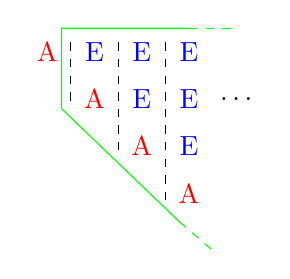
\begin{tikzpicture}[scale = 0.6]
    \foreach \y in {0,...,2}
    {\foreach \x in {\y,...,2}
      \draw (\x+1, -\y) node[color=blue]{E} ;
    }
    \foreach \x in {0,...,3} \draw (\x, -\x) node[color=red]{A} ;
    \draw(4,-1) node{$\ldots$};
    \draw[style = dashed](0.5,0.2) -- (0.5,-1.2);
    \draw[style = dashed](1.5,0.2) -- (1.5,-2.2);
    \draw[style = dashed, thin](2.5,0.2) -- (2.5,-3.2);
    
    \draw[color=green]  (3,0.5) -- (0.3,0.5) -- (0.3,
    -1.2)  -- (2.8,-3.6);
    \draw[color=green, dashed]  (3,0.5) -- (4,0.5);
    \draw[color=green, dashed]  (2.8,-3.6) -- (3.5,-4.2);
  \end{tikzpicture}\\[-2ex]
  \caption{Dividing a triangle into columns}
  \label{fig:visu_col}
\end{figure}

\vspace{-1ex}
If we cut the triangle into the first column and the rest, we get one
element of $A$ and a ``\emph{trapezium}'', with an uppermost row
solely consisting of $E$'s. In order not to have to ensure explicitly
by a dependent type that the number of columns is coherent, the
solution is to transform the trapezium into a triangle, integrating
the side diagonal (just above the diagonal) into the diagonal itself,
as shown in \rfig{tri_trap}.
From the left to the right, the lowermost element of $E$ in each
column is paired with the element of $A$ on the diagonal, and the
other elements of $E$ remain untouched.

\begin{figure}[h]
  \centering
  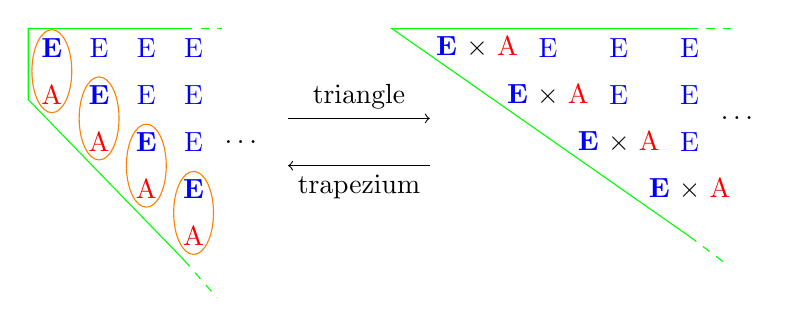
\begin{tikzpicture}[scale = 0.6]
    \foreach \y in {0,...,2}
    {\foreach \x in {\y,...,2}
      \draw (\x+1, -\y) node[color=blue]{E} ;
    }
    \foreach \x in {0,...,3} \draw (\x, -\x-1) node[color=red]{A} ;
    \foreach \x in {0,...,3} \draw (\x, -\x)
    node[color=blue]{\textbf{E}} ;
    \draw(4,-2) node{$\ldots$};

    \foreach \y in {0,...,2}
    {\foreach \x in {\y,...,2}
      \draw (1.5*\x+10.5, -\y) node[color=blue]{E} ;
    }
    \foreach \x in {0,...,3} \draw (1.5*\x+9, -\x)
    node{{\color{blue}\textbf{E}} $\times$ {\color{red} A}} ;
    \draw(14.5,-1.5) node{$\ldots$};
    
    \draw[->] (5,-1.5) to node[swap, auto, above]{triangle}
    (8,-1.5) ; 
    
    \draw[<-] (5,-2.5) to node[swap, auto, below]{trapezium}
    (8,-2.5) ; 

    \draw[color=green] (2.8,0.4) -- (-0.5,0.4) -- (-0.5, -1.1) --
    (2.8,-4.5)  ; 
    \draw[color=green, dashed] (2.8,0.4) -- (3.6,0.4) ; 
    \draw[color=green, dashed] (2.8,-4.5) -- (3.5,-5.3) ; 

    \draw[color=green] (13.5,0.4) -- (7.2,0.4) -- (13.5, -4); 
    \draw[color=green, dashed] (13.5,0.4) -- (14.4,0.4) ; 
    \draw[color=green, dashed] (13.5,-4) -- (14.3,-4.6) ; 

    \draw[color=orange](0, -0.5) ellipse (12pt and 25pt) ;  
    \draw[color=orange](1, -1.5) ellipse (12pt and 25pt) ;  
    \draw[color=orange](2, -2.5) ellipse (12pt and 25pt) ;  
    \draw[color=orange](3, -3.5) ellipse (12pt and 25pt) ;  
  \end{tikzpicture}\\[-2ex]
  \caption{}
  \label{fig:tri_trap}
\end{figure}

\vspace{-1ex}
Following this remark, the triangles can be defined
 theoretically \cite{grossestcspaper}, and in Coq and
Isabelle by the following constructors \cite{types07}:\\[-4ex]
\begin{multicols}{2}
  \begin{prooftree}
    \AxiomC {$a : A$}
    \UnaryInfC{$\sgf\,a : \Trif\,A$}
  \end{prooftree}
  \begin{prooftree}
    \AxiomC {$a : A$}
    \AxiomC {$t : \Trif(E\times A)$}
    \BinaryInfC{$\constrf\,a\,t : \Trif\,A$}
  \end{prooftree}
\end{multicols}

\vspace{-2.5ex}
\begin{remark}
  In this paper, single-lined inference rules denote 
  inductive definitions, double-lined inference rules are for
  coinductive definitions. 
\end{remark}

In more theoretical terms, \Trif{} is modeled as the \emph{least}
solution to the fixed-point equation
$$\Trif\,A=A+ A\times\Trif\,(E\times A)$$
The left summand corresponds to a triangle that only consists of a
single element of $A$ (a singleton), thus ensuring the base case.

The algorithm of redecoration (see work by Uustalu and Vene for
the general
categorical notion  \cite{DBLP:conf/sfp/UustaluV01}) is the following: for a given redecoration rule
$f:\Trif\,A\to B$, it is a function $\redec\,f$ that redecorates
$A$-triangles $t$ (elements of $\Trif\,A$) into $B$-triangles by
applying $f$ to the whole triangle $t$ to obtain the new top element,
and then by successively applying the same operation to the triangle
cut out from the remaining trapezium. This ends in the singleton case
where $f$ is applied to it and the result is turned into a triangle by
applying $\sgf$.  This algorithm only changes the diagonal elements in
$A$ into elements of $B$, as shown in \rfig{redecf}. We do not give
the formal definition of redecoration for finite triangles here.

\begin{figure}[h]
  \centering
  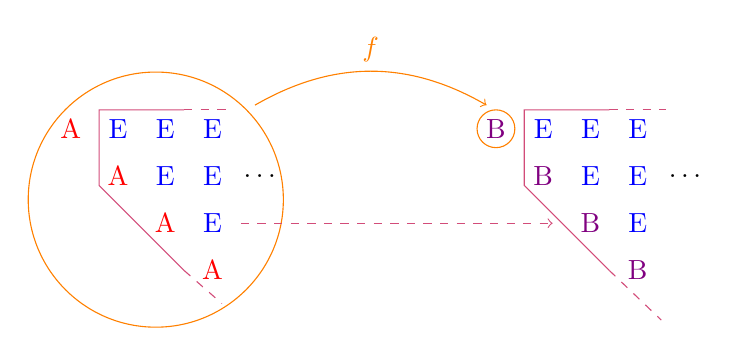
\begin{tikzpicture}[scale = 0.6]
    
    \foreach \y in {0,...,2}
    {\foreach \x in {\y,...,2}
      \draw (\x+1, -\y) node[color=blue]{E} ;
    }
    \foreach \x in {0,...,3} \draw (\x, -\x) node[color=red]{A} ;
    \draw(4,-1) node{$\ldots$};

    \foreach \y in {0,...,2}
    {\foreach \x in {\y,...,2}
      \draw (\x+10, -\y) node[color=blue]{E} ;
    }
    \foreach \x in {0,...,3} \draw (\x+9, -\x) node[color=violet]{B} ;
    \draw(13,-1) node{$\ldots$};
    \draw[color=purple!70]  (2.4, -3) --
    (0.6,-1.2) -- (0.6,0.4) -- (2.4,0.4);
    \draw[color=purple!70, dashed]  (2.4,0.4) -- (3.4,0.4);
    \draw[color=purple!70, dashed]  (2.4,-3) -- (3.2,-3.7);
 
    \draw[color=orange] (1.8,-1.5) circle(2.7cm);

    \draw[color=purple!70]  (11.4, -3) --
    (9.6,-1.2) -- (9.6,0.4) -- (11.4,0.4);
    \draw[color=purple!70, dashed]  (11.4,0.4) -- (12.6,0.4);
    \draw[color=purple!70, dashed]  (11.4,-3) -- (12.5,-4.05);
    
    \draw[color=orange] (9,0) circle(0.4cm);
    
    \draw[->,color = orange] (3.9,0.5) to [bend left] node[auto,
    swap, above]{$f$} (8.8,0.5) ; 

    \draw[->,color = purple!70, dashed] (3.6,-2) to (10.2,-2) ; 
    
  \end{tikzpicture}
  \caption{Redecoration}
  \label{fig:redecf}
\end{figure}

The redecoration for infinite
triangles \cite{grossestcspaper} has not yet been verified. This is
what we intend to do in this paper. 

Reasoning about nested coinductive types naturally rests on
observational equality, just as for ordinary coinductive types, and
since version 8.2, Coq greatly helps in using the rewrite mechanism
for Leibniz equality also for the notion of bisimilarity of infinite
triangular matrices.  With
respect to that notion of equality, redecoration is shown to form a
(sligthly weakened form of) comonad, and its implementation is
compared with an alternative one based on streams of streams.

These new results come with a full formalization in Coq \cite{TYPES11code}, and
limitations of what Coq recognizes as a guarded definition make the
theoretical development more challenging, but we still obtained smooth
results without an excessive overhead that would be imposed by a naive
dualization of the formalization for the finite triangles \cite{types07}.

In \rsect{original}, inspired by the previous theoretical development
\cite{grossestcspaper}, we introduce the dual to the definition of
finite triangles \cite{types07}. We present it with all the
tools necessary to define redecoration. We then propose a definition
for the redecoration algorithm on these infinite triangles and add
further tools and properties. In \rsect{streams}, we change the point
of view in the observation of the triangles. We give an alternative
definition for the infinite triangles, considering this new approach,
and provide various tools. We also show that this new representation
is equivalent to the previous one. Finally, we propose two ways of
defining redecoration, trying always to simplify and generalize our
definitions and show their adequation with previous definitions.

Since the results are fully formalized in the current version of Coq,
hence ensuring complete and sound proofs, we took the liberty to write the paper in
standard mathematical and type-theoretic language and also to omit
most proofs. Therefore, it should be accessible without any specific
knowledge about Coq. For the study of the development
\cite{TYPES11code}, the Coq'Art book \cite{coqart} should mostly suffice, but
the (type) class mechanism \cite{DBLP:conf/tphol/SozeauO08} and the
revised setoid rewriting mechanism based on it have to be consulted
elsewhere -- by default in the Coq Reference Manual \cite{MC}.


%%% Local Variables:
%%% mode: latex
%%% TeX-master: "coredec"
%%% End:
